\newpage
\section{Revisão Teórica}
\subsection{Conversor Buck}
Os conversores cc/cc controlam o fluxo de energia entre dois sistemas de corrente contínua, sendo que, a topologia Buck pode ser utilizada para diminuir a tensão de entrada do circuito. Este conversor, Buck, representado na figura \ref{f_topo_buck}, onde a fonte de tensão contínua é representada por Ve, S representa a chave (geralmente do tipo MOSFET), o indutor é representado por L, D um diodo de roda-livre, um capacitor C e a carga representado por um resistor R com tensão Vs. O circuito em questão é, então, analisado em 2 estados, quando a chave está aberta e quando a chave está fechada.

\begin{figure}[H]
	\centering
	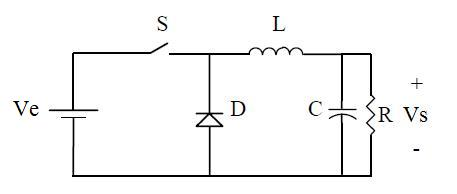
\includegraphics[scale=0.5]{Imagens/topo_buck.jpg}
	\caption{Esquemático de um conversor cc/cc do tipo Buck.}
	\label{f_topo_buck}
\end{figure}

\subsection{Chave fechada}
Em um primeiro momento a chave S está fechada e o diodo D está inversamente polarizado e pode ser desconsiderado, C está sendo carregado, como mostra a figura \ref{f_etp1}.

\begin{figure}[H]
	\centering
	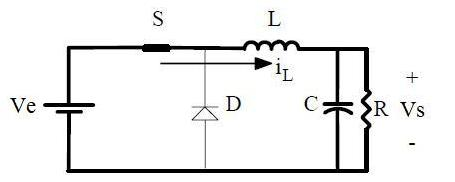
\includegraphics[scale=0.5]{Imagens/etp1.jpg}
	\caption{Conversor Buck com a chave fechada.}
	\label{f_etp1}
\end{figure}

Para não ocorrer a saturação do indutor L, a tensão $V_L$ deve possuir média zero. Ou seja:
\[V_{Lmed} = 0 V.\]

Através da analise de malha, temos que:

\begin{equation}
(V_s - V_e)D.T = V_s(T-D.T).
\label{e_malha1}
\end{equation}

Onde T é o período de chaveamento e D é a razão cíclica.

Expandindo a equação \ref{e_malha1}, temos:
\[V_e.D.T - V_s.D.T = V_s.T - V_s.D.T\]
\[V_e.D.T = V_s.T\]
\[V_e.D = V_s\]
\begin{equation}
\frac{V_s}{V_e} = D
\label{e_ganho}
\end{equation}

A equação \ref{e_ganho} nos dá o ganho do circuito para um conversor Buck ideal.

\subsection{Chave aberta}
Para a chave aberta (figura \ref{f_etp2}), a corrente do indutor é forçada a passar pelo diodo de roda livre. Note que a tensão $V_s$ é mantida pelo capacitor C.

\begin{figure}[H]
	\centering
	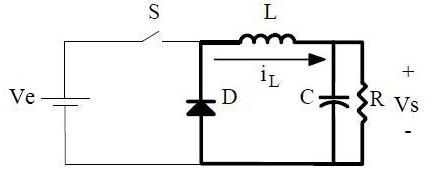
\includegraphics[scale=0.5]{Imagens/etp2.jpg}
	\caption{Conversor Buck com a chave aberta.}
	\label{f_etp2}
\end{figure}

Sendo assim, podemos encontrar a tensão máxima na chave e no indutor.

\begin{equation}
V_L = V_s
\end{equation}

\begin{equation}
V_{ch} = V_e
\end{equation}